\documentclass[10pt,a4paper,oneside]{article}
\usepackage[utf8]{inputenc}
\usepackage{draftwatermark} % 设置水印
\SetWatermarkText{DNV Group} % 水印内容
\usepackage{amsmath}
\usepackage{amsfonts}
\usepackage{amssymb}
\usepackage{graphicx}
\usepackage{breqn}
\usepackage{tikz} % system block diagram
\usepackage{textcomp}
\usetikzlibrary{shapes,arrows} % system block diagram
\usepackage{booktabs}
\usepackage[framed,numbered,autolinebreaks,useliterate]{mcode} % matlab code block
\author{Yangang Cao}
\newcommand{\degree}{^\circ}
\tikzset{
	delay/.style    = {draw, thick, rectangle, minimum height = 3em,
		minimum width = 3em},
	sum/.style      = {draw, circle, node distance = 2cm}, 
	prod/.style     = {draw, circle, node distance = 2cm},
	input/.style    = {coordinate}, % Input
	output/.style  = {coordinate} % Output
}
% Defining string as labels of certain blocks.
\newcommand{\product}{$\displaystyle \times$}
\newcommand{\delay}{\large$z^{-1}$}
\begin{document}

\title{Filter Design}
\maketitle 

The signal can be seen as a set of partials having different frenquencies and amplitudes. The filter can modify the amplitude of partials according to their frenquency.

\section{Basic Filters}
\subsection{Filter classification in the frenquency domain}

The various types of filters can be defined according to the following classification:

\begin{itemize}
	\item {\bfseries Lowpass (LP)} filters select low frenquencies up to the cut-off frenquency $f_c$ and attenuate frenquencies higher than $f_c$. Additionally, a resonance may amply frenquencies around $f_c$.
	\item {\bfseries Highpass (HP)} filters select high frenquencies higher than $f_c$ and attenuate frenquencies below $f_c$, possibly with a resonance around $f_c$.
	\item {\bfseries Bandpass (BP)} filters select frenquencies between a lower cut-off frenquency $f_{cl}$ and a higher cut-off frenquency $f_{ch}$. Frenquencies below $f_{cl}$ and frenquencies higher than $f_{ch}$ are attenuated.
	\item {\bfseries Bandreject (BR)} filters attenuate frenquencies between a lower cut-off frenquency $f_{cl}$ and a higher cut-off frenquency $f_{ch}$. Frenquencies below $f_{cl}$ and frenquencies higher than $f_{ch}$ are passed.
\end{itemize}

The lowpass with resonance is very often used in computer music to simulate an acoustical resonating structure; the highpass filter can remove undesired very low frequencies; the bandpass can produce effects such as the imitation of a telephone line or of a mute on an acoustical instrument; the bandreject can divide the audible spectrum into two bands that seem to be uncorrelated.

\subsection{Canonical filters}
There are various ways to implement a filter, the simplest being the canonical filter, as shown in following figure for a second-order filter, which can be implemented by the defference equations
\[
x(n) = u(n) - a_1x(n-1) - a_2x(n-2)
\]
\[
y(n) = b_0x(n) + b_1x(n-1) + b_2x(n-2),
\]



\begin{center}
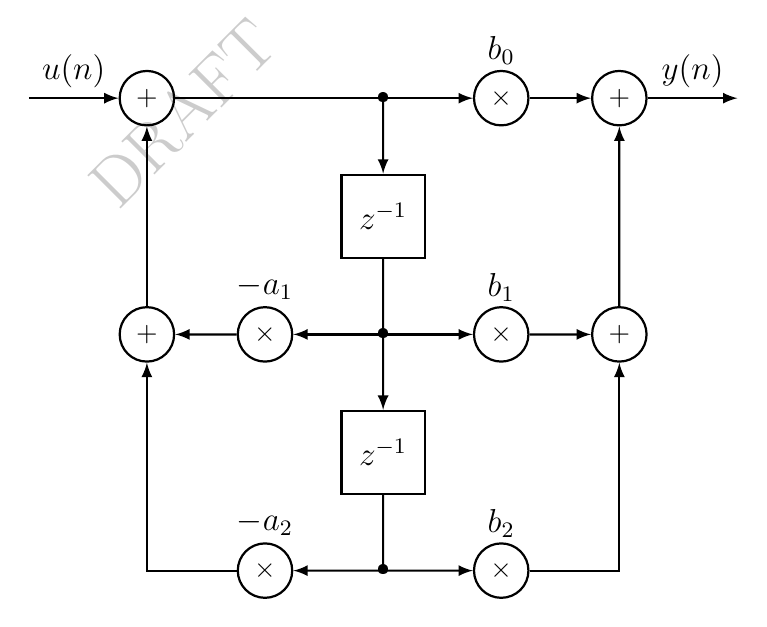
\begin{tikzpicture}[auto, thick, node distance=0.6cm, >=latex, scale = 0.75]
\draw
% Drawing the blocks of first filter 
node at (0,0)[sum] (s1) {$+$}
node at (6,0)[prod] (p1) {\product} node[above of = p1] {\large$b_0$}
node at (8,0)[sum] (s2) {$+$}
node at (4,-2) [delay] (d1) {\delay}
node at (0,-4) [sum] (s3) {$+$}
node at (2,-4) [prod] (p2) {\product} node[above of = p2] {\large$-a_1$}
node at (6,-4) [prod] (p3) {\product} node[above of = p3] {\large$b_1$}
node at (8,-4) [sum] (s4) {$+$}
node at (4,-6) [delay] (d2) {\delay}
node at (2,-8) [prod] (p4) {\product} node[above of = p4] {\large$-a_2$}
node at (6,-8) [prod] (p5) {\product} node[above of = p5] {\large$b_2$};

\draw[->](-2,0) -- node {\large$u(n)$}(s1);
\draw[->](s1) -- node {} (p1);
\draw[->](p1) -- node {} (s2);
\draw[->](s2) -- node {\large$y(n)$} (10,0);
\draw[->](4,0) -- node {} (d1);
\draw[->](d1) -- node {} (d2);
\draw[<->](p2) -- node {} (p3);
\draw[->](p2) -- node {} (s3);
\draw[->](s3) -- node {} (s1);
\draw[->](p3) -- node {} (s4);
\draw[->](s4) -- node {} (s2);
\draw[-](d2) -- node {} (4,-8);
\draw[<->](p4) -- node {} (p5);
\draw[->](p4) -| node {} (s3);
\draw[->](p5) -| node {} (s4);

\draw
node at (4,0) {\textbullet} 
node at (4,-4){\textbullet}
node at (4,-8){\textbullet};
\end{tikzpicture}
\end{center}
and leads to the transfer function by setting $a_2 = b_2 = 0$, this reduces to a first-order filter which, can be used to implement an allpass, lowpass or highpass with the coefficients of following table
\begin{center}
	\begin{tabular}{cccc}
	\toprule  %添加表格头部粗线
	 & {$b_0$}&{$b_1$}&{$a_1$}\\
	\midrule  %添加表格中横线
	Lowpass&K/(K+1)& K/(K+1) & (K-1)/(K+1)\\
	Highpass& 1/(K+1)& -1/(K+1) & (K-1)/(K+1)\\
	Allpass&(K-1)/(K+1)&1&(K-1)/(K+1)\\
	\bottomrule %添加表格底部粗线
	\end{tabular}
\end{center}
where $K$ depends on the cut-off frequency $f_c$ by
\[
K=\tan(\pi f_c/f_S).
\]

\subsection{First-order allpass-based filters}

In this section we introduce a special class of parametric filter structures for lowpass, highpass, bandpass and bandreject filter functions. These filter structures are easily tunable by changing only one or two coefficients. They play an important role for real-time control with minimum computational complexity.

The basis for parametric first- and second-order IIR filters is the first- and second-order allpass filter. We will first discuss the first-order allpass and show simple lowpass and highpass filters, which consist of a tunable allpass filter together with a direct path.

A first-order allpass filter is given by the transfer function
\[
A(z) = \frac{z^{-1} + c}{1 + cz^{-1}}
\]
\[
c = \frac{\tan(\pi f_c/f_S) - 1}{\tan(\pi f_c/f_S) + 1},
\]
and the corresponding difference equation
\[
x(n) = u(n) - cx(n-1)
\]
\[
y(n) = cx(n) + x(n-1),
\]
which can be realized by the following block diagram.
\begin{center}
	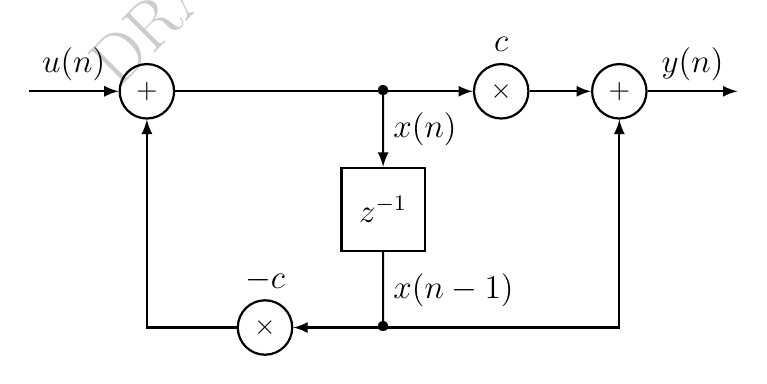
\begin{tikzpicture}[auto, thick, node distance=0.6cm, >=latex, scale = 0.75]
	\draw
	% Drawing the blocks of first filter 
	node at (0,0)[sum] (s1) {$+$}
	node at (6,0)[prod] (p1) {\product} node[above of = p1] {\large$c$}
	node at (8,0)[sum] (s2) {$+$}
	node at (4,-2) [delay] (d1) {\delay}
	node at (2,-4) [prod] (p2) {\product} node[above of = p2] {\large$-c$};
	
	\draw[->](-2,0) -- node {\large$u(n)$}(s1);
	\draw[->](s1) -- node {} (p1);
	\draw[->](p1) -- node {} (s2);
	\draw[->](s2) -- node {\large$y(n)$} (10,0);
	\draw[->](4,0) -- node {\large$x(n)$} (d1);
	\draw[->](p2) -| node {} (s1);
	\draw[-](d1) -- node {\large$x(n-1)$} (4,-4);
	\draw[<->](p2) -| node {} (s2);
	
	\draw
	node at (4,0) {\textbullet} 
	node at (4,-4){\textbullet};
	
	\end{tikzpicture}
\end{center}
A first-order allpass filter implementation can be obtained by the following {\bfseries Matlab} code.
\begin{lstlisting}
function y = firstallpassunit(audio, para)
% Applies a allpass filter to the input signal.
% para is the normalized cut-off frequency in (0,1)
c = (tan(pi*para/2)-1) / (tan(pi*para/2)+1);
x = 0;
x_1 = 0;
for n = 1:length(audio)
	x_1 = -c * x+ audio(n);
	y(n) = (1-c^2) * x + c * audio(n);
	x = x_1;
end
\end{lstlisting}

\subsection{First-order low/highpass filters}
A first-order lowpass/highpass filter can be achieved by adding or subtracting (+/--) the output signal from the input signal of a first-order allpass filter.The transfer function of a lowpass/highpass filter is then given by

\[
H(z) = \frac{1}{2}(1 \pm A(z))\quad(LP/HP+/-)
\]
\[
A(z) = \frac{z^{-1} + c}{1 + cz^{-1}}
\]
\[
c = \frac{\tan(\pi f_c/f_S) - 1}{\tan(\pi f_c/f_S) + 1}.
\]

where a tunable first-order allpass $A(z)$ with tuning parameter $c$ is used. The plus sign (+) denotes the lowpass operation and the minus sign (--) the highpass operation. The block diagram in following figure represents the operations involved in performing the low/highpass filtering. 
\begin{center}
	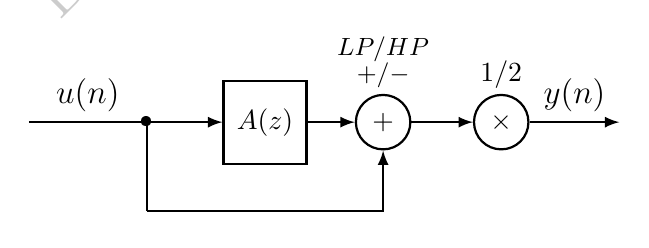
\begin{tikzpicture}[auto, thick, node distance=0.6cm, >=latex, scale = 0.75]
	\draw
	node at (2,0)[delay] (d1) {$A(z)$}
	node at (4,0)[sum] (s1) {$+$} 
	node[above of = s1]{\small$+/-$} node[above of=s1,above=1]{\small{$LP/HP$}}
	node at (6,0) [prod] (p1) {\product} node[above of = p1]{$1/2$};
	
	\draw[-](-2,0) -- node {\large$u(n)$}(0,0);
	\draw[->](0,0) -- node {} (d1);
	\draw[->](d1) -- node {} (s1);
	\draw[->](s1) -- node {} (p1);
	\draw[->](p1) -- node {\large$y(n)$} (8,0);
	\draw[-](0,0) -- node {} (0,-1.5);
	\draw[->](0,-1.5) -| node {} (s1);
	
	\draw
	node at (0,0) {\textbullet};
	
	\end{tikzpicture}
\end{center}

A first-order lowpass filter implementation can be obtained by the following {\bfseries Matlab} code.


\begin{lstlisting}
function y = aplowpassunit(audio, para)
% Applies a lowpass filter to the input signal.
% para is the normalized cut-off frequency in (0,1)
c = (tan(pi*para/2)-1) / (tan(pi*para/2)+1);
x = 0;
x_1 = 0;
for n = 1:length(audio)
	x_1 = -c * x+ audio(n);
	y(n) = ((1-c^2)/2) * x + (1+c)/2 * audio(n);
	x = x_1;   
end
\end{lstlisting}

A first-order highpass filter implementation can be obtained by the following {\bfseries Matlab} code.
\begin{lstlisting}
function y = aphighpassunit(audio, para)
% Applies a highpass filter to the input signal.
% para is the normalized cut-off frequency in (0,1)
c = (tan(pi*para/2)-1) / (tan(pi*para/2)+1);
x = 0;
x_1 = 0;
for n = 1:length(audio)
	x_1 = -c * x+ audio(n);
	y(n) = ((c^2-1)/2) * x + (1-c)/2 * audio(n);
	x = x_1;  
end
\end{lstlisting}
\subsection{Second-order allpass-based filters}
The implementation of tunable bandpass and bandreject filters can be achieved with a second-order allpass filter. The transfer function of a second-order allpass filter is given by
\[
A(z) = \frac{-c + d(1-c)z^{-1} + z^{-2}}{1 + d(1-c)z^{-1} - cz^{-2}}
\]
\[
c = \frac{\tan(\pi f_b/f_S) - 1}{\tan(\pi f_b/f_S) + 1}
\]
\[
d = -\cos(2\pi f_c/f_S),
\]
with the corresponding difference equatons
\[
x(n) = u(n) - d(1-c)x(n-1) + cx(n-2)
\]
\[
y(n) = -cx(n) + d(1-c)x(n-1) + x(n-2).
\]
The parameter $d$ adjusts the center frequency and the parameter $c$ the bandwidth. The
magnitude response is again equal to one and the phase response approaches ${-360\degree}$ for high
frequencies. The cut-off frequency $f_c$ determines the point on the phase curve where the phase response passes ${-180\degree}$. The width or slope of the phase transition around the cut-off frequency is controlled by the bandwidth parameter $f_b$. The following block diagram shows the second-order allpass filter.
\begin{center}
	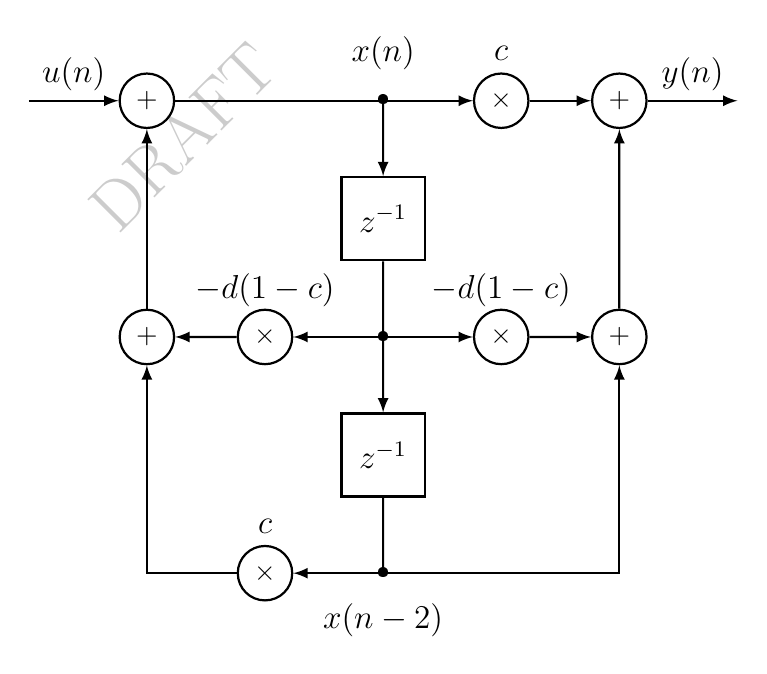
\begin{tikzpicture}[auto, thick, node distance=0.6cm, >=latex, scale = 0.75]
	\draw
	% Drawing the blocks of first filter 
	node at (0,0)[sum] (s1) {$+$}
	node at (6,0)[prod] (p1) {\product} node[above of = p1] {\large$c$}
	node at (8,0)[sum] (s2) {$+$}
	node at (4,-2) [delay] (d1) {\delay}
	node at (0,-4) [sum] (s3) {$+$}
	node at (2,-4) [prod] (p2) {\product} node[above of = p2] {\large$-d(1-c)$}
	node at (6,-4) [prod] (p3) {\product} node[above of = p3] {\large$-d(1-c)$}
	node at (8,-4) [sum] (s4) {$+$}
	node at (4,-6) [delay] (d2) {\delay}
	node at (2,-8) [prod] (p4) {\product} node[above of = p4] {\large$c$}
	 ;
	
	\draw[->](-2,0) -- node {\large$u(n)$}(s1);
	\draw[->](s1) -- node {} (p1);
	\draw[->](p1) -- node {} (s2);
	\draw[->](s2) -- node {\large$y(n)$} (10,0);
	\draw[->](4,0) -- node {} (d1);
	\draw[->](d1) -- node {} (d2);
	\draw[<->](p2) -- node {} (p3);
	\draw[->](p2) -- node {} (s3);
	\draw[->](s3) -- node {} (s1);
	\draw[->](p3) -- node {} (s4);
	\draw[->](s4) -- node {} (s2);
	\draw[-](d2) -- node {} (4,-8);
	\draw[<->](p4) -| node {} (s4);
	\draw[->](p4) -| node {} (s3);
	
	\draw
	node at (4,0)(n1) {\textbullet} node[above of = n1]{\large$x(n)$}
	node at (4,-4){\textbullet}
	node at (4,-8)(n2){\textbullet} node[below of = n2]{\large$x(n-2)$};
	\end{tikzpicture}
\end{center}
A second-order allpass filter implementation can be obtained by the following {\bfseries Matlab} code.
\begin{lstlisting}
function y = secondallpassunit(audio, para)
% Applies a allpass filter to the input signal.
% para(1) is the normalized center frequency in (0,1), i.e. 2*fc/fs.
% para(2) is the normalized bandwidth in (0,1) i.e. 2*fb/fs.
c = (tan(pi*para(2)/2)-1) / (tan(pi*para(2)/2)+1);
d = -cos(pi*para(1));
x = [0; 0];
x_1 = 0;
A = [-d*(1-c), c; 1, 0];
B = [1; 0];
C = [d*(1-c^2), 1-c^2];
D = -c;
for n=1:length(audio)
	x_1 = A * x + B * audio(n);
	y(n) = C * x + D * audio(n);
	x = x_1;
end
\end{lstlisting}
\subsection{Second-order bandpass/bandreject filters}
Second-order bandpass and bandreject filters can be described by the following transfer function
\[
H(z) = \frac{1}{2}[1 \mp A(z)]\quad(BP/BR-/+)
\]
\[
A(z) = \frac{-c + d(1-c)z^{-1} + z^{-2}}{1 + d(1-c)z^{-1} - cz^{-2}}
\]
\[
c = \frac{\tan(\pi f_b/f_S) - 1}{\tan(\pi f_b/f_S) + 1}
\]
\[
d = -\cos(2\pi f_c/f_S),
\]
where a tunable second-order allpass $A(z)$ with tuning parameters $c$ and $d$ is used. The minus sign (-) denotes the bandpass operation and the plus sign (+) the bandreject operation. The block diagram in following figure represents the operations involved in performing the bandpass/bandreject filtering.
\begin{center}
	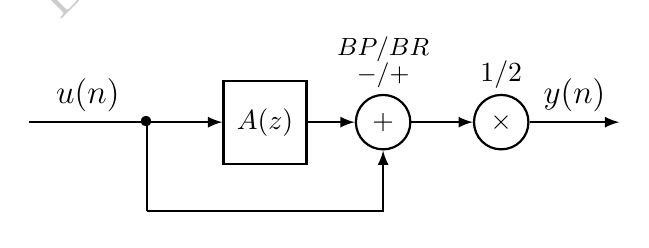
\begin{tikzpicture}[auto, thick, node distance=0.6cm, >=latex, scale = 0.75]
	\draw
	node at (2,0)[delay] (d1) {$A(z)$}
	node at (4,0)[sum] (s1) {$+$} 
	node[above of = s1]{\small$-/+$} node[above of=s1,above=1]{\small{$BP/BR$}}
	node at (6,0) [prod] (p1) {\product} node[above of = p1]{$1/2$};
	
	\draw[-](-2,0) -- node {\large$u(n)$}(0,0);
	\draw[->](0,0) -- node {} (d1);
	\draw[->](d1) -- node {} (s1);
	\draw[->](s1) -- node {} (p1);
	\draw[->](p1) -- node {\large$y(n)$} (8,0);
	\draw[-](0,0) -- node {} (0,-1.5);
	\draw[->](0,-1.5) -| node {} (s1);
	
	\draw
	node at (0,0) {\textbullet};
	\end{tikzpicture}
\end{center}
A second-order bandpass filter implementation can be obtained by the following {\bfseries Matlab} code.
\begin{lstlisting}
function y = apbandpassunit(audio, para)
% Applies a bandpass filter to the input signal.
% para(1) is the normalized center frequency in (0,1), i.e. 2*fc/fs.
% para(2) is the normalized bandwidth in (0,1) i.e. 2*fb/fs.
c = (tan(pi*para(2)/2)-1) / (tan(pi*para(2)/2)+1);
d = -cos(pi*para(1));
x = [0; 0];
x_1 = 0;
A = [-d*(1-c), c; 1, 0];
B = [1; 0];
C = [d*(c^2-1)/2, (c^2-1)/2];
D = (1+c)/2;
for n=1:length(audio)
	x_1 = A * x + B * audio(n);
	y(n) = C * x + D * audio(n);
	x = x_1;
end
\end{lstlisting}
A second-order bandreject filter implementation can be obtained by the following {\bfseries Matlab} code.
\begin{lstlisting}
function y = apbandrejectunit(audio, para)
% Applies a bandreject filter to the input signal.
% para(1) is the normalized center frequency in (0,1), i.e. 2*fc/fs.
% para(2) is the normalized bandwidth in (0,1) i.e. 2*fb/fs.
c = (tan(pi*para(2)/2)-1) / (tan(pi*para(2)/2)+1);
d = -cos(pi*para(1));
x = [0; 0];
x_1 = 0;
A = [-d*(1-c), c; 1, 0];
B = [1; 0];
C = [d*(1-c^2)/2, (1-c^2)/2];
D = (1-c)/2;
for n=1:length(audio)
	x_1 = A * x + B * audio(n);
	y(n) = C * x + D * audio(n);
	x = x_1;
end
\end{lstlisting}
\section{Equalizers}
In contrast to low/highpass and bandpass/reject filters, which attenuate the audio spectrum above or below a cut-off frequency, equalizers shape the audio spectrum by enhancing certain frequency bands while others remain unaffected. They are typically built by a series connection of first-and second-order shelving and peak filters, which are controlled independently.

Shelving filters boost or cut the low- or high-frequency bands with the parameters cut-off frequency $f_c$ and gain $G$. Peak filters boost or cut mid-frequency bands with parameters center frequency $f_c$, bandwidth $f_b$ and gain $G$. One often-used filter type is the constant $Q$ peak filter. The $Q$ factor is defined by the ratio of the bandwidth to center frequency $Q = fb/fc$. The center frequency of peak filters is then tuned while keeping the $Q$ factor constant. This means that the bandwidth is increased when the center frequency is increased and vice versa.
\subsection{Shelving filters}
Similar to the first-order lowpass/highpass filters described in Section 1.4, first-order low/high
frequency shelving filters can be constructed based on a first-order allpass, yielding the
transfer function
\[
H(z) = 1 + \frac{H_0}{2}[1 \pm A(z)]\quad(LF/HF+/-)
\]
with the first-order allpass
\[
A(z) = \frac{z^{-1} + c_{B/C}}{1 + c_{B/C}z^{-1}}.
\]

The block diagram in following figure shows a first-order low/high-frequency shelving filter, the part of $A(z)$ can be reviewed in Section 1.3,
\begin{center}
	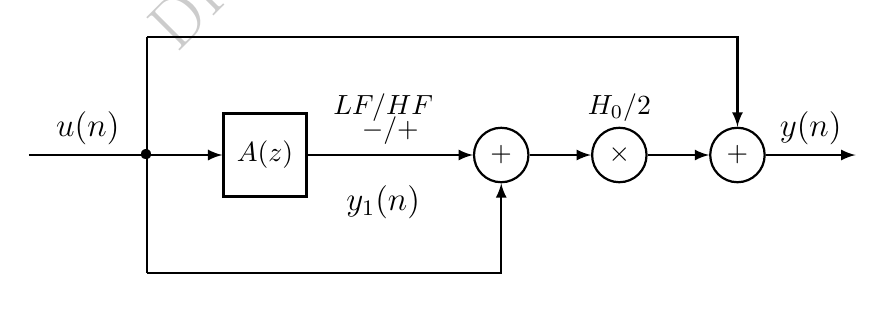
\begin{tikzpicture}[auto, thick, node distance=0.6cm, >=latex, scale = 0.75]
	\draw
	node at (2,0)[delay] (d1) {$A(z)$}
	node at (6,0)[sum] (s1) {$+$}
	node at (8,0)[prod](p1){$\times$} node[above of = p1]{$H_0/2$}
	node at (10,0)[sum](s2){$+$}
	node at (4,0)(n1){}
	node[above of = n1]{$LF/HF$} node[below of =n1]{\large$y_1(n)$}
	;
	
	\draw[-](-2,0) -- node {\large$u(n)$}(0,0);
	\draw[->](0,0) -- node {} (d1);
	\draw[->](d1) -- node {$-/+$} (s1);
	\draw[-](0,0) -- node {} (0,-2);
	\draw[->](0,-2) -| node {} (s1);
	\draw[->](s1) -- node {} (p1);
	\draw[->](p1) -- node {} (s2);
	\draw[->](s2) -- node {\large$y(n)$} (12,0);
	\draw[-](0,0) -- node {} (0,2);
	\draw[->](0,2) -| node {} (s2);
	
	\draw
	node at (0,0) {\textbullet};
	\end{tikzpicture}
\end{center}
which leads to the difference equations
\[
x(n) = u(n) - c_{B/C}x(n-1)
\]
\[
y_1(n) = c_{B/C}x(n) + x(n-1)
\]
\[
y(n) = \frac{H_0}{2}[u(n) \pm y_1(n)] + u(n).
\]
The gain $G$ in dB for low/high frequencies can be adjusted by the parameter
\[
H_0 = V_0 - 1\quad \mbox{with} \quad V_0 = 10^{G/20}.
\]
The cut-off frenquency parameters, $c_B$ for boost and $c_C$ for cut, for a first-order low-frequency shelving filter can be calculated as
\[
c_B = \frac{\tan(\pi f_c/f_S) - 1}{\tan(\pi f_c/f_S) + 1}
\]
\[
c_C = \frac{\tan(\pi f_c/f_S) - V_0}{\tan(\pi f_c/f_S) + V_0},
\]
and for a high-frequency shelving filter as
\[
c_B = \frac{\tan(\pi f_c/f_S) - 1}{\tan(\pi f_c/f_S) + 1}
\]
\[
c_C = \frac{V_0\tan(\pi f_c/f_S) - 1}{V_0\tan(\pi f_c/f_S) + 1}.
\]
An implementation of low-frenquency shelving filter is given in following {\bfseries Matlab} code
\begin{lstlisting}
function y = lowshelvingunit(audio, para)
% Applies a low-frequency shelving filter to the input signal.
% para(1) is the normalized cut-off frequency in (0,1), i.e. 2*fc/fs
% para(2) is the gain in dB
V0 = 10^(para(2)/20); H0 = V0 - 1;
if para(2) >= 0
	c = (tan(pi*para(1)/2)-1) / (tan(pi*para(1)/2)+1);     % boost
else
	c = (tan(pi*para(1)/2)-V0) / (tan(pi*para(1)/2)+V0);   % cut
end
x = 0;
x_1 = 0;
for n=1:length(audio)
	x_1 = -c * x + audio(n);
	y(n) = H0 / 2 * (1-c^2) * x + [H0 / 2 * (1+c) + 1] * audio(n);
	x = x_1;
end
\end{lstlisting}
An implementation of high-frenquency shelving filter is given in following {\bfseries Matlab} code
\begin{lstlisting}
function y = highshelvingunit(audio, para)
% Applies a high-frequency shelving filter to the input signal.
% para(1) is the normalized cut-off frequency in (0,1), i.e. 2*fc/fS
% para(2) is the gain in dB
V0 = 10^(para(2)/20); H0 = V0 - 1;
if para(2) >= 0
c = (tan(pi*para(1)/2)-1) / (tan(pi*para(1)/2)+1);     % boost
else
c = (tan(pi*para(1)/2)-V0) / (tan(pi*para(1)/2)+V0);   % cut
end
x = 0;
x_1 = 0;
for n=1:length(audio)
	x_1 = -c * x + audio(n);
	y(n) = H0/2 * (c^2-1) * x + (H0/2 * (1-c) + 1) * audio(n);
	x = x_1;
end
\end{lstlisting}
\subsection{Peak filters}
Similarly, a second-order peak filter is given by the transfer function
\[
H(z) = 1 + \frac{H_0}{2}[1 - A_2(z)],
\]
where
\[
A_2(z) = \frac{-c_{B/C} + d(1 - c_{B/C})z^{-1} + z^{-2}}{1 + d(1 - c_{B/C})z^{-1} - c_{B/C}z^{-2}}
\]
is a second-order allpass filter. The block diagram in following figure shows the second-order peak filter, the part of $A_2(z)$ can be reviewed in Section 1.5,
\begin{center}
	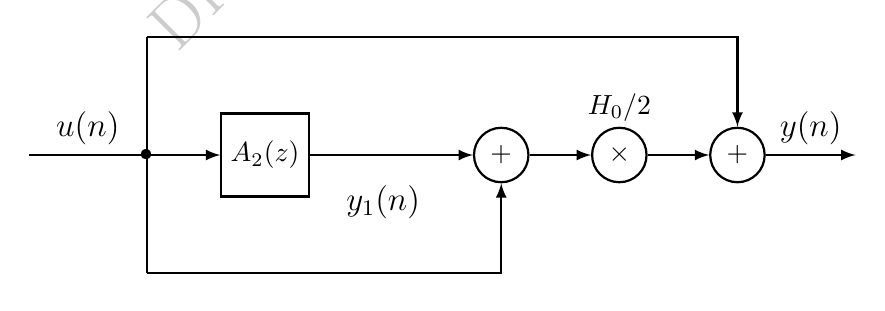
\begin{tikzpicture}[auto, thick, node distance=0.6cm, >=latex, scale = 0.75]
	\draw
	node at (2,0)[delay] (d1) {$A_2(z)$}
	node at (6,0)[sum] (s1) {$+$}
	node at (8,0)[prod](p1){$\times$} node[above of = p1]{$H_0/2$}
	node at (10,0)[sum](s2){$+$}
	node at (4,0)(n1){}
	node[below of =n1]{\large$y_1(n)$}
	;
	
	\draw[-](-2,0) -- node {\large$u(n)$}(0,0);
	\draw[->](0,0) -- node {} (d1);
	\draw[->](d1) -- node {} (s1);
	\draw[-](0,0) -- node {} (0,-2);
	\draw[->](0,-2) -| node {} (s1);
	\draw[->](s1) -- node {} (p1);
	\draw[->](p1) -- node {} (s2);
	\draw[->](s2) -- node {\large$y(n)$} (12,0);
	\draw[-](0,0) -- node {} (0,2);
	\draw[->](0,2) -| node {} (s2);
	
	\draw
	node at (0,0) {\textbullet};
	\end{tikzpicture}
\end{center}
which leads to the difference equations
\[
x(n) = u(n) - d(1 - c_{B/C})x(n - 1) + c_{B/C}x(n - 2)
\]
\[
y_1(n) = -c_{B/C}x(n) + d(1 - c_{B/C})x(n - 1) + x(n - 2)
\]
\[
y(n) = \frac{H_0}{2}[u(n) - y_1(n)] + u(n).
\]
The center frenquency parameter $d$ and the coefficient $H_0$ are given by
\[
d = -\cos(2\pi f_c/f_S)
\]
\[
V_0 = H(e^{j2\pi f_c/f_S}) = 10^{G/20}
\]
\[
H_0 = V_0 - 1.
\]
The bandwidth $f_b$ is adjusted through the parameters $c_B$ and $c_C$ for boost and cut given by
\[
c_B = \frac{\tan(\pi f_b/f_S) - 1}{\tan(\pi f_b/f_S) + 1}
\]
\[
c_C = \frac{\tan(\pi f_b/f_S) - V_0}{\tan(\pi f_b/f_S) + V_0}.
\]
A possible peak filter implementation using this approach is given in the following {\bfseries Matlab} code.
\begin{lstlisting}
function y = peakfiltunit(audio, para)
% Applies a peak filter to the input signal.
% para(1) is the normalized center frequency in (0,1), i.e. 2*fc/fs.
% para(2) is the normalized bandwidth in (0,1), i.e. 2*fb/fs.
% prar(3) is the gain in dB.
V0 = 10^(para(3)/20); H0 = V0 - 1;
if para(3) >= 0
	c = (tan(pi* para(2)/2)-1) / (tan(pi* para(2)/2)+1);     % boost
else
	c = (tan(pi* para(2)/2)-V0) / (tan(pi* para(2)/2)+V0);   % cut
end;
d = -cos(pi*para(1));
x = [0; 0];
x_1 = 0;
A = [-d*(1-c), c; 1, 0];
B = [1; 0];
C = [H0/2*(c^2-1)*d, H0/2*(c^2-1)];
D = [H0/2*(1+c) + 1];
for n=1:length(audio)
	x_1 = A * x + B * audio(n);
	y(n) = C * x + D * audio(n);
	x = x_1;
end
\end{lstlisting}
\end{document}
